%%%%%%%%%%%%%%%%%%%%%%%%%%%%%%%%%%%%%%%%%%%%%%%%%%%%%%%%%%%%%%%%%%%%%%%%%%%%%%%%%%%%
% Configuración de Paquetes
\documentclass{article}
\usepackage[framemethod=TikZ]{mdframed}
\usepackage{booktabs}
\usepackage{float}
\usepackage{scrextend}
\usepackage{titletoc}
\usetikzlibrary{calc}
\usepackage[margin=1in]{geometry} 
\usepackage{amsmath,amsthm,amssymb,amsfonts, fancyhdr, color, comment, graphicx, environ}
\usepackage{xcolor}
\usepackage{mdframed}
\usepackage[shortlabels]{enumitem}
\usepackage{indentfirst}
\usepackage{hyperref}
\usepackage{listings}
\usepackage{karnaugh-map}
\usepackage{booktabs}
\usepackage{geometry}
\hypersetup{
    colorlinks=true,
    linkcolor=blue,
    filecolor=magenta,      
    urlcolor=blue,
}
\setlength{\headheight}{1.5cm}
\renewcommand{\qed}{\quad\qedsymbol}
 % Incluir configuración de paquetes y encabezado
\renewcommand{\familydefault}{\sfdefault}
%%%%%%%%%%%%%%%%%%%%%%%%%%%%%%%%%%%%%%%%%%%%%%%%%%%%%%%%%%%%%%%%%%%%%%%%%%%%%%%%%%%%

\fancypagestyle{mipagina}{
    \fancyhf{} % Limpiar encabezado y pie de página
    \fancyhead[L]{Pedro Villar} % Nombre a la izquierda
    \fancyhead[C]{\rightmark} % Texto al centro 
    \fancyhead[R]{Alg. y E.D 2} % Texto a la derecha
    \fancyfoot[C]{\thepage} % Número de página al centro
    \renewcommand{\headrulewidth}{0.4pt} % Grosor de la línea horizontal en el encabezado
}

\pagestyle{mipagina}
\mdfsetup{skipabove=\topskip,skipbelow=\topskip}

% Box de Definición
\newcounter{def}[section]

\NewDocumentEnvironment{defi}{o}{%
    \stepcounter{def}%
    \begin{mdframed}[
        frametitle={%
            \begin{tikzpicture}[baseline=(current bounding box.east),outer sep=0pt]
                \node[anchor=east,rectangle,fill=blue!20,inner xsep=5pt] at (0,0) {\strut\IfValueTF{#1}{Definición~\thedef:~#1}{Definición~\thedef}};
            \end{tikzpicture}%
        },
        innertopmargin=5pt,
        linecolor=blue!20,
        linewidth=2pt,
        topline=true,
        frametitleaboveskip=-\ht\strutbox, % Ajuste de espacio entre título y contenido
        frametitlealignment={\hspace{5pt}}, % Ajuste de espacio entre el borde del frame y el título
    ]
}{%
    \end{mdframed}%
}

% Box de ejemplos
\newcounter{ejemplo}[section]

\NewDocumentEnvironment{ejemplo}{o}{%
    \stepcounter{ejemplo}%
    \begin{mdframed}[
        frametitle={%
            \begin{tikzpicture}[baseline=(current bounding box.east),outer sep=0pt]
                \node[anchor=east,rectangle,fill=brown!30,inner xsep=5pt] at (0,0) {\strut\IfValueTF{#1}{Ejemplo~\theejemplo:~#1}{Ejemplo~\theejemplo}};
            \end{tikzpicture}%
        },
        innertopmargin=5pt,
        linecolor=brown!30,
        linewidth=2pt,
        topline=true,
        frametitleaboveskip=-\ht\strutbox, % Ajuste de espacio entre título y contenido
        frametitlealignment={\hspace{5pt}}, % Ajuste de espacio entre el borde del frame y el título
    ]
}{%
    \end{mdframed}%
}

% Entorno para Métodos (color verde)
\newcounter{metodo}[section]
\NewDocumentEnvironment{metodo}{o}{%
    \stepcounter{metodo}%
    \begin{mdframed}[
        frametitle={%
            \begin{tikzpicture}[baseline=(current bounding box.east),outer sep=0pt]
                \node[anchor=east,rectangle,fill=green!30,inner xsep=5pt] at (0,0) {\strut\IfValueTF{#1}{Método~\themetodo:~#1}{Método~\themetodo}};
            \end{tikzpicture}%
        },
        innertopmargin=5pt,
        linecolor=green!30,
        linewidth=2pt,
        topline=true,
        frametitleaboveskip=-\ht\strutbox, % Ajuste de espacio entre título y contenido
        frametitlealignment={\hspace{5pt}}, % Ajuste de espacio entre el borde del frame y el título
    ]
}{%
    \end{mdframed}%
}

% Entorno para Observaciones (color amarillo más oscuro)
\newcounter{observacion}[section]
\NewDocumentEnvironment{observacion}{o}{%
    \stepcounter{observacion}%
    \begin{mdframed}[
        frametitle={%
            \begin{tikzpicture}[baseline=(current bounding box.east),outer sep=0pt]
                \node[anchor=east,rectangle,fill=yellow!50,inner xsep=5pt] at (0,0) {\strut\IfValueTF{#1}{Observación~\theobservacion:~#1}{Observación~\theobservacion}};
            \end{tikzpicture}%
        },
        innertopmargin=5pt,
        linecolor=yellow!50,
        linewidth=2pt,
        topline=true,
        frametitleaboveskip=-\ht\strutbox, % Ajuste de espacio entre título y contenido
        frametitlealignment={\hspace{5pt}}, % Ajuste de espacio entre el borde del frame y el título
    ]
}{%
    \end{mdframed}%
}

% Entorno para Ejercicio
\newcounter{ejer}[section]
\NewDocumentEnvironment{ejer}{o}{%
    \stepcounter{ejer}%
    \begin{mdframed}[
        frametitle={%
            \begin{tikzpicture}[baseline=(current bounding box.east),outer sep=0pt]
                \node[anchor=east,rectangle,fill=black!30,inner xsep=5pt] at (0,0) {\strut\IfValueTF{#1}{Ejercicio~\theejer:~#1}{Ejercicio~\theejer}};
            \end{tikzpicture}%
        },
        innertopmargin=5pt,
        linecolor=black!30,
        linewidth=2pt,
        topline=true,
        frametitleaboveskip=-\ht\strutbox, % Ajuste de espacio entre título y contenido
        frametitlealignment={\hspace{5pt}}, % Ajuste de espacio entre el borde del frame y el título
    ]
}{%
    \end{mdframed}%
}

\newenvironment{solution}
    {\textit{Solución:}}
    {}


\newcounter{pascalcode}[section]

\renewcommand{\thepascalcode}{\arabic{section}.\arabic{pascalcode}}

\lstdefinelanguage{pascal-like}{
  morekeywords={var, type, tuple, enumerate, fi, ret, downto, where, proc, fun, in, out, if, then, else, while, do, for, to, end, od},
  morecomment=[s]{\{-}{-\}},
  morestring=[b]",
  sensitive=true,
  keywordstyle=\color{orange},
  commentstyle=\color{green!70!black},
  stringstyle=\color{blue!70!black},
  numbers=left,
  numberstyle=\tiny\color{gray},
  alsoletter={:,=,+,-,*,>,<,(,)},
  morekeywords=[2]{:,=,+,-,*,>,<,(,),&,&&,||,!,!=,==},
  keywordstyle=[2]{\color{blue}},
  literate={:=}{{\textcolor{blue}{:=}}}2,
  morekeywords=[3]{nat, array, of, int, real, bool, char}, 
  keywordstyle=[3]{\color{green!40!black}},
}

\lstnewenvironment{pascallike}[1][]{
  \refstepcounter{pascalcode}
  \lstset{
    language=pascal-like,
    numbers=left,
    numberstyle=\tiny\color{gray},
    captionpos=b,
    #1
  }
}{\phantomsection\addcontentsline{lol}{section}{Código \thepascalcode}}


%Configuraciones adicionales
\binoppenalty=\maxdimen 
\relpenalty=\maxdimen 

\begin{document}

%%%%%%%%%%%%%%%%%%%%%%%%%%%%%%%%%%%%%%%%%%%%%
%Condiguracion de la portada
\begin{titlepage}
    \begin{tikzpicture}[remember picture,overlay,inner sep=0,outer sep=0]
         \draw[blue!70!black,line width=4pt] ([xshift=-1.5cm,yshift=-2cm]current page.north east) coordinate (A)--([xshift=1.5cm,yshift=-2cm]current page.north west) coordinate(B)--([xshift=1.5cm,yshift=2cm]current page.south west) coordinate (C)--([xshift=-1.5cm,yshift=2cm]current page.south east) coordinate(D)--cycle;
    
         \draw ([yshift=0.5cm,xshift=-0.5cm]A)-- ([yshift=0.5cm,xshift=0.5cm]B)--
         ([yshift=-0.5cm,xshift=0.5cm]B) --([yshift=-0.5cm,xshift=-0.5cm]B)--([yshift=0.5cm,xshift=-0.5cm]C)--([yshift=0.5cm,xshift=0.5cm]C)--([yshift=-0.5cm,xshift=0.5cm]C)-- ([yshift=-0.5cm,xshift=-0.5cm]D)--([yshift=0.5cm,xshift=-0.5cm]D)--([yshift=0.5cm,xshift=0.5cm]D)--([yshift=-0.5cm,xshift=0.5cm]A)--([yshift=-0.5cm,xshift=-0.5cm]A)--([yshift=0.5cm,xshift=-0.5cm]A);
    
    
         \draw ([yshift=-0.3cm,xshift=0.3cm]A)-- ([yshift=-0.3cm,xshift=-0.3cm]B)--
         ([yshift=0.3cm,xshift=-0.3cm]B) --([yshift=0.3cm,xshift=0.3cm]B)--([yshift=-0.3cm,xshift=0.3cm]C)--([yshift=-0.3cm,xshift=-0.3cm]C)--([yshift=0.3cm,xshift=-0.3cm]C)-- ([yshift=0.3cm,xshift=0.3cm]D)--([yshift=-0.3cm,xshift=0.3cm]D)--([yshift=-0.3cm,xshift=-0.3cm]D)--([yshift=0.3cm,xshift=-0.3cm]A)--([yshift=0.3cm,xshift=0.3cm]A)--([yshift=-0.3cm,xshift=0.3cm]A);
    
    \end{tikzpicture}
    \begin{center}
        \vspace{7pt}
        
        \textbf{Pedro Villar}
        
        \vspace{7pt}
    
    \end{center}
    \vspace{15pt}
    \begin{center}
        
\includegraphics[scale=0.25]{famaf-logo.jpg}
        
        \vspace{50pt}
        \fontsize{18pt}{17pt}\selectfont 
        \textbf{Notas de Clase} 
        
        \vspace{7pt}
        \textbf{Algoritmos y Estructuras de Datos 2}

        \vspace{5pt}
        \textbf{Teórico Práctico}
    \end{center}
    
    \vspace{15pt}
    
    \vspace{10pt}
    \begin{center}
        \textbf{\date{today}}
    \end{center}
    \vspace{25pt} % Espacio vertical adicional
    
    \begin{center}
        \textbf{Primer Cuatrimestre 2024}
    \end{center}
\end{titlepage}
%%%%%%%%%%%%%%%%%%%%%%%%%%%%%%%%%%%%%%%%%%%%%

%%%%%%%%%%%%%%%%%%%%%%%%%%%%%%%%%%%%%%%%%%%%%
%Condiguracion del índice
\clearpage
\newpage
\thispagestyle{empty}
\section*{Información de la materia}
\subsection*{Profesores}
\begin{itemize}
    \item \textbf{Teórico:} Emanuel Gunther, Luque Franco, Bustos Facundo, Vilela Demetrio y Zigarán Gonzalo.
    \item \textbf{Laboratorio:} Avalos Santiago, Cabral Juan, Canchi Sergio, Gadea Alejandro, Molina Matias, Peralta Gonzalo, Ramos Leandro y Rocchietti Marco.
\end{itemize}
\subsection*{Régimen de regularidad y promoción}
\begin{itemize}
    \item \textbf{Regularidad:} Para regularizar la materia, se tienen que aprobar con nota mayor a $4$ ambos parciales.
    \item \textbf{Promoción:} Para promocionar la materia, se tienen que aprobar con nota mayor o igual a $6$ ambos parciales y tener un promedio mayor o igual a $7$.
\end{itemize}
\textit{No hay recuperatorios para promoción.}
\subsection*{Bibliografía}
Se utilizará el material de la cátedra que está aca \href{https://wiki.cs.famaf.unc.edu.ar/doku.php?id=algo2:main:2022}{FAMAF Wiki}.
\newpage


\thispagestyle{empty}
\begin{center}
    \huge \textbf{Índice de Contenido}
\end{center}

\noindent\makebox[\linewidth]{\rule{\textwidth}{0.4pt}}

\startcontents
\printcontents{}{1}{}
\newpage
%%%%%%%%%%%%%%%%%%%%%%%%%%%%%%%%%%%%%%%%%%%%%

\section{Repaso de Arreglos}

\subsection{Arreglos multidimensionales}
Los arreglos multidimensionales en C son estructuras de datos que permiten almacenar elementos en más de una dimensión. Por ejemplo, un arreglo unidimensional es similar a una lista, mientras que un arreglo bidimensional es similar a una tabla o una matriz.

\subsubsection{Declaración}

1. \textbf{Declaración directa:}
\begin{verbatim}
int matriz[3][3];
\end{verbatim}
Esto declara una matriz de enteros de 3x3. Los elementos de la matriz no se inicializan y contendrán valores basura hasta que se les asigne un valor explícitamente.

2. \textbf{Inicialización explícita:}
\begin{verbatim}
int matriz[3][3] = {
    {1, 2, 3},
    {4, 5, 6},
    {7, 8, 9}
};
\end{verbatim}
Aquí se declara e inicializa una matriz de 3x3 con valores específicos.

3. \textbf{Usando typedef:}
\begin{verbatim}
typedef int ArregloBidimensional[3][3];
ArregloBidimensional matriz;
\end{verbatim}
Esto declara un tipo `ArregloBidimensional`, que luego se usa para declarar una matriz de 3x3 llamada `matriz`.

4. \textbf{Arreglo de punteros:}
\begin{verbatim}
int *matriz[3];
for (int i = 0; i < 3; i++) {
    matriz[i] = malloc(3 * sizeof(int));
}
\end{verbatim}
En este caso, se declara un arreglo de punteros a enteros. Luego, en un bucle, se asigna memoria dinámica para cada fila de la matriz.

5. \textbf{Usando punteros dobles:}
\begin{verbatim}
int **matriz;
matriz = malloc(3 * sizeof(int *));
for (int i = 0; i < 3; i++) {
    matriz[i] = malloc(3 * sizeof(int));
}
\end{verbatim}
Aquí, `matriz` es un puntero doble que apunta a un bloque de memoria que contiene punteros a enteros. Luego, en un bucle, se asigna memoria dinámica para cada fila de la matriz.

Es importante tener en cuenta que las diferentes formas de declarar arreglos multidimensionales tienen implicaciones diferentes, especialmente en lo que respecta a la asignación de memoria y la gestión de punteros. Selecciona el método que mejor se adapte a tus necesidades y ten en cuenta la gestión adecuada de la memoria para evitar fugas de memoria y comportamientos inesperados.

\subsection{Acceso a elementos}
Por ejemplo, un arreglo bidimensional se puede visualizar como una tabla con filas y columnas. Para acceder a un elemento específico en un arreglo multidimensional, necesitas especificar los índices correspondientes a cada dimensión del arreglo.

\begin{verbatim}
#include <stdio.h>

int main() {
    // Declaración e inicialización de un arreglo bidimensional 2x3
    int arreglo[2][3] = {
        {1, 2, 3},
        {4, 5, 6}
    };

    // Acceso a elementos individuales
    printf("Elemento en la fila 0, columna 0: %d\n", arreglo[0][0]);
    printf("Elemento en la fila 1, columna 2: %d\n", arreglo[1][2]);

    return 0;
}
\end{verbatim}

En este ejemplo, \texttt{arreglo} es un arreglo bidimensional de tamaño 2x3. Para acceder a un elemento específico, utilizamos la sintaxis \texttt{arreglo[i][j]}, donde \texttt{i} representa el índice de la fila y \texttt{j} representa el índice de la columna. Recuerda que en C, los índices comienzan desde cero, por lo que el primer elemento de la matriz tiene índices \texttt{[0][0]}.

El mismo concepto se aplica a arreglos multidimensionales con más de dos dimensiones. Por ejemplo, para un arreglo tridimensional, necesitarías especificar tres índices: \texttt{arreglo[i][j][k]}, donde \texttt{i}, \texttt{j} y \texttt{k} representan las coordenadas en cada dimensión respectivamente.

\subsection{Paso de arreglos multidimensionales a funciones}
Cuando pasas un arreglo multidimensional a una función en C, debes tener en cuenta que la función no recibe un puntero a un arreglo multidimensional, sino un puntero a un arreglo unidimensional. Esto se debe a que los arreglos multidimensionales en C se almacenan en memoria de forma contigua, lo que significa que se pueden tratar como arreglos unidimensionales.

\begin{verbatim}
#include <stdio.h>

// Función que recibe un puntero a un arreglo multidimensional
void imprimirMatriz(int (*matriz)[3]) {
    for (int i = 0; i < 3; i++) {
        for (int j = 0; j < 3; j++) {
            printf("%d ", matriz[i][j]);
        }
        printf("\n");
    }
}

int main() {
    int matriz[3][3] = {
        {1, 2, 3},
        {4, 5, 6},
        {7, 8, 9}
    };

    // Llamada a la función
    imprimirMatriz(matriz);

    return 0;
}
\end{verbatim}

En este ejemplo, la función \texttt{imprimirMatriz} recibe un puntero a un arreglo multidimensional de 3x3. La sintaxis \texttt{int (*matriz)[3]} indica que la función recibe un puntero a un arreglo de 3 elementos (es decir, una fila de la matriz). Dentro de la función, podemos tratar el puntero como un arreglo unidimensional de 3 elementos, lo que nos permite acceder a los elementos de la matriz.

\subsection{Juego del gato (Tic-Tac-Toe) en C}

\subsubsection{Inclusión de Bibliotecas:}

\begin{verbatim}
#include <stdio.h>
#include <stdbool.h>
\end{verbatim}

Se incluyen las bibliotecas estándar de C, \texttt{<stdio.h>} para entrada/salida estándar y \texttt{<stdbool.h>} para usar el tipo de datos booleano y los valores \texttt{true} y \texttt{false}.

\subsubsection{Declaración de Funciones:}

\begin{verbatim}
bool has_free_cell(char board[3][3]);
bool get_winner(char board[3][3]);
\end{verbatim}

Se declaran las funciones \texttt{has\_free\_cell} y \texttt{get\_winner}, que son responsables de verificar si hay celdas libres en el tablero y de determinar si hay un ganador, respectivamente.

\subsubsection{Función Principal (\texttt{main()}):}

\begin{verbatim}
int main() {
    char board[3][3] = {
        {'-', '-', '-'}, 
        {'-', '-', '-'}, 
        {'-', '-', '-'}};
    char player = 'X'; // Jugador actual (inicia con 'X')

    while (has_free_cell(board) && !get_winner(board)) {
        // ...
    }

    // Verificación del ganador o empate
    // ...
    return 0;
}
\end{verbatim}

Se declara e inicializa una matriz \texttt{board} de 3x3 que representa el tablero del juego, inicializando todas las celdas con el carácter \texttt{'-'}. Se declara la variable \texttt{player} para almacenar el símbolo del jugador actual, que comienza con \texttt{'X'}. Se inicia un bucle \texttt{while} que continuará mientras haya celdas libres en el tablero y no haya un ganador. Dentro del bucle, se imprime el tablero, se solicita al jugador que ingrese su jugada y se actualiza el tablero con la jugada del jugador actual. Luego se cambia el jugador. Después de salir del bucle, se verifica si hay un ganador o si hay un empate y se imprime el resultado correspondiente.

\subsubsection{Función \texttt{has\_free\_cell()}:}

\begin{verbatim}
bool has_free_cell(char board[3][3]) {
    // ...
}
\end{verbatim}

Esta función recibe el tablero como argumento y verifica si hay alguna celda libre (\texttt{'-'}) en el tablero. Utiliza dos bucles \texttt{while} anidados para iterar sobre todas las celdas del tablero. Si encuentra al menos una celda libre, devuelve \texttt{true}; de lo contrario, devuelve \texttt{false}.

\subsubsection{Función \texttt{get\_winner()}:}

\begin{verbatim}
bool get_winner(char board[3][3]) {
    // ...
}
\end{verbatim}

Esta función recibe el tablero como argumento y verifica si hay un ganador. Comprueba todas las filas, columnas y diagonales para ver si tienen el mismo símbolo (\texttt{'X'} o \texttt{'O'}) y no son \texttt{'-'}. Si encuentra un ganador, devuelve \texttt{true}; de lo contrario, devuelve \texttt{false}.

\subsubsection{Código completo}

\begin{verbatim}
    #include <stdio.h>
    #include <stdbool.h>
    
    bool has_free_cell(char board[3][3]);
    bool get_winner(char board[3][3]);
    
    int main() {
        char board[3][3] = {
            {'-', '-', '-'}, 
            {'-', '-', '-'}, 
            {'-', '-', '-'}};
        // Cruz y círculo para jugar
        char player = 'X';
        
        while (has_free_cell(board) && !get_winner(board)) {
            // Imprimir el tablero
            printf("Tablero:\n");
            int i = 0;
            while (i < 3) {
                int j = 0;
                while (j < 3) {
                    printf("%c ", board[i][j]);
                    j++;
                }
                printf("\n");
                i++;
            }
            // Pedir la jugada
            int pos, x, y;
            printf("Ingrese la posición de la jugada: ");
            scanf("%d", &pos);
            switch (pos)
            {
            case 0:
                x = 0;
                y = 0;
                break;
            case 1:
                x = 0;
                y = 1;
                break;
            case 2:
                x = 0;
                y = 2;
                break;
            case 3:
                x = 1;
                y = 0;
                break;
            case 4:
                x = 1;
                y = 1;
                break;
            case 5:
                x = 1;
                y = 2;
                break;
            case 6:
                x = 2;
                y = 0;
                break;
            case 7:
                x = 2;
                y = 1;
                break;
            case 8:
                x = 2;
                y = 2;
                break;        
            default:
                printf("Posición inválida\n");
            }
            if (board[x][y] != '-') {
                printf("Posición ocupada\n");
                continue;
            }
            board[x][y] = player;
            // Cambiar de jugador
            if (player == 'X') {
                player = 'O';
            } else {
                player = 'X';
            }
        } 
        if (get_winner(board)) {
            if (player == 'X') {
                player = 'O';
            } else {
                player = 'X';
            }
            printf("¡Felicidades! Ganó el jugador %c\n", player);
        } else {
            printf("¡Empate!\n");
        }
    
        return 0;
    }
    
    bool has_free_cell(char board[3][3]) {
        int i = 0;
        int j = 0;
        while (i < 3) {
            while (j < 3) {
                if (board[i][j] == '-') {
                    return true;
                }
                j++;
            }
            i++;
        }
        return false;
    }
    
    bool get_winner(char board[3][3]) {
        int i = 0;
        while (i < 3) {
            if (board[i][0] == board[i][1] && board[i][1] == board[i][2] && board[i][0] != '-') {
                return true;
            }
            if (board[0][i] == board[1][i] && board[1][i] == board[2][i] && board[0][i] != '-') {
                return true;
            }
            i++;
        }
        if (board[0][0] == board[1][1] && board[1][1] == board[2][2] && board[0][0] != '-') {
            return true;
        }
        if (board[0][2] == board[1][1] && board[1][1] == board[2][0] && board[0][2] != '-') {
            return true;
        }
        return false;
    }    
\end{verbatim}

Este es un ejemplo de un juego del gato (Tic-Tac-Toe) en C. El programa utiliza una matriz de 3x3 para representar el tablero del juego y permite a dos jugadores alternar turnos para marcar las celdas del tablero. El programa verifica si hay un ganador o si hay un empate después de cada jugada. El juego continúa hasta que haya un ganador o hasta que no haya celdas libres en el tablero. El código utiliza funciones para verificar si hay celdas libres en el tablero y para determinar si hay un ganador. También incluye la lógica para imprimir el tablero y solicitar las jugadas de los jugadores.

\newpage
\subsection{Tic-Tac-Toe para tamaño n}
Ahora vamos a ver una posible solución al ejercicio de crear un programa que emule un tictactoe para un tablero de tamaño n. La solución que se presenta a continuación es una de las muchas posibles, y se basa en la implementación de un tablero de tamaño n x n, y en la verificación de las condiciones de victoria para un tablero de tamaño variable.

\subsubsection{Inclusión de Bibliotecas:}
\begin{verbatim}
#include <stdbool.h>
#include <stdio.h>
\end{verbatim}

Se incluyen las bibliotecas estándar de C necesarias para el programa, una para el tipo de dato booleano (\texttt{<stdbool.h>}) y otra para entrada/salida estándar (\texttt{<stdio.h>}). 

\subsubsection{Declaración de Constantes:}
\begin{verbatim}
#define SIZE 4
\end{verbatim}
Se define una constante \texttt{SIZE} que representa el tamaño del tablero. En este caso, el tablero será de tamaño 4x4, pero se podrá cambiar y sigue funcionando para cualquier tamaño.

\subsubsection{Función \texttt{has\_free\_cell()}:}
\begin{verbatim}
bool has_free_cell(char board[SIZE][SIZE]) {
    int i = 0;
    while(i < SIZE) {
        int j = 0;
        while(j < SIZE) {
            if(board[i][j] == '-') {
                return true;
            }
            j++;
        }
        i++;
    }
    return false;
}
\end{verbatim}

La función busca una celda libre en la matriz \texttt{board}, representada por el carácter `'-'`. La lógica de funcionamiento es la siguiente:

\begin{enumerate}
    \item Se inicializa un contador $i$ en 0.
    \item Se inicia un bucle \texttt{while} exterior que itera mientras $i$ sea menor que \texttt{SIZE}. Esto permite recorrer todas las filas de la matriz.
    \item Dentro de este bucle exterior, se inicializa un contador $j$ en 0.
    \item Se inicia un bucle \texttt{while} interior que itera mientras $j$ sea menor que \texttt{SIZE}. Esto permite recorrer todas las columnas de la matriz para la fila actual.
    \item Dentro de este bucle interior, se verifica si el elemento en la posición $(i, j)$ de la matriz \texttt{board} es igual a `'-'`. Si lo es, significa que hay una celda libre, por lo que la función devuelve \texttt{true}.
    \item Si no se encuentra una celda libre en la fila actual, se incrementa $j$ para pasar a la siguiente columna.
    \item Una vez que se ha recorrido toda la fila actual, se incrementa $i$ para pasar a la siguiente fila y se reinicia $j$ a 0 para empezar a recorrer las columnas de esa fila.
    \item Este proceso se repite hasta que se recorren todas las filas y columnas de la matriz.
    \item Si no se encuentra ninguna celda libre en toda la matriz, la función devuelve \texttt{false} al final.
\end{enumerate}

\subsubsection{Función \texttt{get\_winner()}:}

\begin{verbatim}
    bool get_winner(char board[SIZE][SIZE]) {
        int i = 0;
        while(i < SIZE) {
            int j = 0;
            char first = board[i][0];
            while(j < SIZE) {
                if(board[i][j] != first || first == '-') {
                    break;
                }
                j++;
            }
            if(j == SIZE) {
                return true;
            }
            i++;
        }
    
        i = 0;
        while(i < SIZE) {
            int j = 0;
            char first = board[0][i];
            while(j < SIZE) {
                if(board[j][i] != first || first == '-') {
                    break;
                }
                j++;
            }
            if(j == SIZE) {
                return true;
            }
            i++;
        }
    
        char first = board[0][0];
        i = 0;
        while(i < SIZE) {
            if(board[i][i] != first || first == '-') {
                break;
            }
            i++;
        }
        if(i == SIZE) {
            return true;
        }
    
        first = board[0][SIZE - 1];
        i = 0;
        while(i < SIZE) {
            if(board[i][SIZE - 1 - i] != first || first == '-') {
                break;
            }
            i++;
        }
        if(i == SIZE) {
            return true;
        }
    
        return false;
    }
\end{verbatim}

La función \texttt{get\_winner}, busca determinar si hay un ganador en el juego representado por la matriz \texttt{board} de tamaño \texttt{SIZE} por \texttt{SIZE} (donde \texttt{SIZE} es una constante definida en otro lugar del código). La función busca ganadores en tres posibles direcciones: horizontal, vertical y diagonal.

\begin{enumerate}
    \item La función comienza recorriendo todas las filas de la matriz \texttt{board}. En cada fila, verifica si todos los elementos son iguales al primer elemento de la fila y si ese elemento es diferente de '-' (que indica una celda vacía). Si esto es cierto, devuelve \texttt{true}, indicando que hay un ganador.
    \item Luego, la función recorre todas las columnas de la matriz \texttt{board}. En cada columna, verifica si todos los elementos son iguales al primer elemento de la columna y si ese elemento es diferente de '-'. Si se cumple esta condición, devuelve \texttt{true}.
    \item Después, la función verifica la diagonal principal de la matriz, es decir, los elementos donde el índice de fila es igual al índice de columna. Si todos los elementos en esta diagonal son iguales al primer elemento de la matriz y ese elemento es diferente de '-', devuelve \texttt{true}.
    \item Finalmente, la función verifica la otra diagonal de la matriz (de arriba a la derecha hacia abajo a la izquierda). Si todos los elementos en esta diagonal son iguales al primer elemento de la matriz y ese elemento es diferente de '-', devuelve \texttt{true}.
\end{enumerate}

Si en ninguno de estos casos se encuentra un ganador, la función devuelve \texttt{false}, indicando que no hay un ganador en el juego.

\subsubsection{Función Principal (\texttt{main()}):}

\begin{verbatim}
    int main(){
    char board[SIZE][SIZE];
    int i = 0;
    while(i < SIZE) {
        int j = 0;
        while(j < SIZE) {
            board[i][j] = '-';
            j++;
        }
        i++;
    }
    // Cruz y círculo para jugar
    char player = 'X';

    while(has_free_cell(board) && !get_winner(board)) {
        // Imprimir el tablero
        i = 0;
        while(i < SIZE) {
            int j = 0;
            while(j < SIZE) {
                printf("%c ", board[i][j]);
                j++;
            }
            printf("\n");
            i++;
        }

        // Pedir la jugada
        int position;
        printf("Jugador %c, ingrese la posición: ", player);
        scanf("%d", &position);

        // Verificar que se inserte una posición válida
        int x = position / SIZE;
        int y = position % SIZE;
        if(x < 0 || x >= SIZE || y < 0 || y >= SIZE || board[x][y] != '-') {
            printf("Posición inválida o ya ocupada, intente de nuevo.\n");
            continue;
        }

        // Realizar la jugada y cambiar de jugador
        board[x][y] = player;
        player = (player == 'X') ? 'O' : 'X';
    }
    
    // Corroborar si hay ganador
    if (get_winner(board)) {
        if (player == 'X') {
            player = 'O';
        } else {
            player = 'X';
        }
        printf("¡Felicidades! Ganó el jugador %c\n", player);
    } else {
        printf("¡Empate!\n");
    }
    return 0;
}
\end{verbatim}

La función principal (\texttt{main()}) es el punto de entrada del programa. En este caso, el programa implementa un juego de tres en raya (Tic-Tac-Toe). A continuación se explica la lógica de la función:

\begin{enumerate}
    \item Se declara una matriz bidimensional \texttt{board} de tamaño \texttt{SIZE} por \texttt{SIZE} para representar el tablero del juego.
    \item Se inicializa el tablero, rellenándolo con el carácter `'-'`, indicando que todas las celdas están vacías.
    \item Se establece el jugador actual como `'X'`, que será el primer jugador en realizar una jugada.
    \item Se inicia un bucle que continuará mientras haya celdas libres en el tablero y no haya un ganador.
    \item Dentro del bucle, se imprime el tablero actual.
    \item Se solicita al jugador actual que ingrese la posición donde desea realizar su jugada.
    \item Se verifica que la posición ingresada sea válida y esté libre en el tablero. Si no lo es, se muestra un mensaje de error y se solicita una nueva posición.
    \item Si la posición es válida, se realiza la jugada colocando el símbolo del jugador actual en la posición correspondiente del tablero.
    \item Se cambia el jugador actual para que el otro jugador pueda realizar su jugada en el siguiente ciclo del bucle.
    \item Una vez que el bucle termina (debido a un ganador o un empate), se verifica si hay un ganador en el tablero. Si hay un ganador, se imprime un mensaje felicitando al jugador ganador. Si no hay ganador, se imprime un mensaje indicando que hubo un empate.
    \item La función retorna 0 para indicar que el programa se ejecutó correctamente.
\end{enumerate}

Esta función implementa la lógica principal del juego, gestionando las jugadas de los jugadores, la validación de las posiciones y la determinación del ganador o empate.

\section{Ordenación elemental}
El problema de ordenar un conjunto de elementos es uno de los problemas más estudiados en la historia de la computación. Existen numerosos algoritmos para resolver este problema, cada uno con sus propias características y desventajas. En esta sección estudiaremos el algoritmo de ordenación más sencillo (pero no el más rápido), cuyo procedimiento es el siguiente:

\begin{enumerate}
    \item \textbf{Selecciona} el menor de todos, lo intercambia con el elemento que se encuentra en la primera posición.
    \item \textbf{Selecciona} el menor de los restantes, lo intercambia con el elemento que se encuentra en la segunda posición. 
    \item \textbf{Selecciona} el menor de los restantes, lo intercambia con el elemento que se encuentra en la tercera posición. 
    \item ... y así sucesivamente hasta que el conjunto esté ordenado.  
\end{enumerate}

\subsection{Recurso gráfico}
Para ilustrar el funcionamiento del algoritmo de ordenación por selección, se ha desarrollado un recurso gráfico que permite visualizar el estado del conjunto en cada iteración. Supongamos que se tiene la lista:
\begin{equation*}
    [ \ 9,3,1,3,5,27 \ ]
\end{equation*}
y lo que se busca es aplicar el algoritmo de ordenación por selección.

\begin{figure}[H]
    \centering
    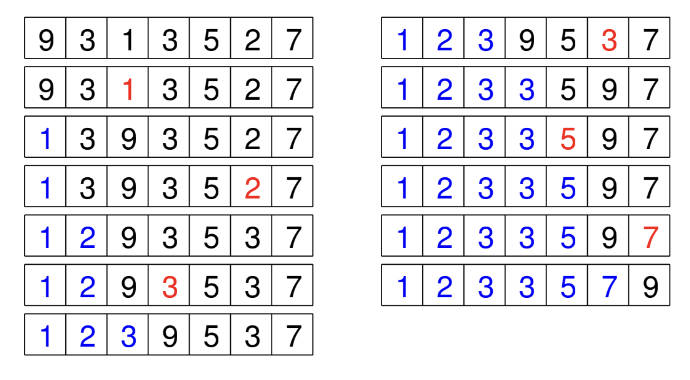
\includegraphics[scale=0.5]{./Images/oedef.png}
    \caption{Paso a paso de la ordenación por selección.}
\end{figure}


\subsection{Código}

\begin{pascallike}
proc selection_sort (in/out a: array[1..n] of T)
    var minp: nat
    for i := 1 to n do
        minp := min_pos_from(a, i)
        swap(a, i, minp) 
    od
end proc

fun min_pos_from (a: array[1..n] of T, i: nat) ret minp: nat
    minp := i
    for j:= i+1 to n do 
        if a[j] < a[minp] then 
            minp:= j 
        fi
    od
end fun

proc swap (in/out a: array[1..n] of T, in i, j: nat)
    var temp: T
    temp := a[i]
    a[i] := a[j]
    a[j] := temp
end proc
\end{pascallike}

Para el algoritmo de ordenación por selección, se ha desarrollado un procedimiento \texttt{selection\_sort} que recibe un arreglo de tamaño $n$ y lo ordena. El procedimiento \texttt{selection\_sort} utiliza dos funciones auxiliares: \texttt{min\_pos\_from} y \texttt{swap}. La función \texttt{min\_pos\_from} recibe un arreglo y una posición, y retorna la posición del menor elemento a partir de la posición dada. La función \texttt{swap} recibe un arreglo y dos posiciones, e intercambia los elementos en dichas posiciones. Se pueden marcar las siguientes observaciones:

\begin{itemize}
    \item \texttt{selection\_sort} utiliza un ciclo \texttt{for} que recorre el arreglo desde la primera posición hasta la última. En cada iteración, se busca el menor elemento a partir de la posición actual y se intercambia con el elemento en la posición actual,
    \item se encuentra una llamada a la función \texttt{min\_pos\_from} que recibe el arreglo y la posición actual, y retorna la posición del menor elemento a partir de la posición actual,
    \item y se recibe tambien una llamada al procedimiento \texttt{swap} que recibe el arreglo y las posiciones actual y la posición del menor elemento, e intercambia los elementos en dichas posiciones,
    \item encontramos una \textbf{comparación} entre elementos de un arreglo, y una \textbf{asignación} de elementos de un arreglo,
    \item la operación que mas se repite es la comparación de elementos de un arreglo, y toda operación se repite a lo sumo de manera proporcional a esa,
    \item como la celda de un arreglo es constante, su costo no depende de cual es la celda o del tamaño del arreglo, por lo que el costo de la operación es constante.
\end{itemize}

\section{Ordenación por inserción}
El algoritmo de ordenación por inserción es un algoritmo sencillo que funciona de la siguiente manera:
\begin{enumerate}
    \item \textbf{Selecciona} el segundo elemento de la lista,
    \item \textbf{verifica} si es menor que el primer elemento, si es así, lo intercambia con el primer elemento,
    \item \textbf{Selecciona} el tercer elemento de la lista,
    \item \textbf{verifica} si es menor que el segundo elemento, si es así, lo intercambia con el segundo elemento, y \textbf{verifica} si es menor que el primer elemento, si es así, lo intercambia con el primer elemento,
    \item y así sucesivamente hasta que el conjunto esté ordenado.
\end{enumerate}

\subsection{Recurso gráfico}
Para ilustrar el funcionamiento del algoritmo de ordenación por inserción, se ha desarrollado un recurso gráfico que permite visualizar el estado del conjunto en cada iteración. Supongamos que se tiene la lista:
\begin{equation*}
    [ \ 9,3,1,3,5,27 \ ]
\end{equation*}

\begin{figure}[H]
    \centering
    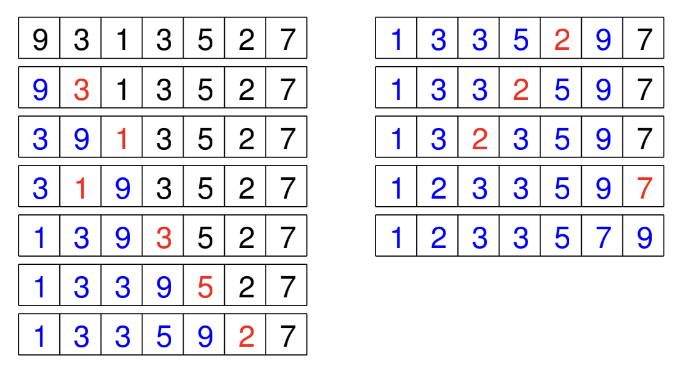
\includegraphics[scale=0.5]{./Images/oedei.png}
    \caption{Paso a paso de la ordenación por inserción.}
\end{figure}

\subsection{Código}

\begin{pascallike}
proc insertion_sort (in/out a: array[1..n] of T)
    for i:= 2 to n do
        insert(a,i)
    od
end proc
proc insert (in/out a: array[1..n] of T, in i: nat)
    var j: nat
    j:= i
    do j > 1 && a[j] < a[j - 1] -> 
        swap(a,j-1,j)
        j:= j-1
    od
end proc
\end{pascallike}

Para el algoritmo de ordenación por inserción, se ha desarrollado un procedimiento \texttt{insertion\_sort} que recibe un arreglo de tamaño $n$ y lo ordena. El procedimiento \texttt{insertion\_sort} utiliza un procedimiento auxiliar \texttt{insert}. El procedimiento \texttt{insert} recibe un arreglo y una posición, y mueve el elemento en la posición dada a la posición correcta. Se puede definir de una forma mas abreviada el algoritmo de ordenación por inserción, como se muestra a continuación:

\begin{pascallike}
proc insertion_sort (in/out a: array[1..n] of T)
    for i:= 2 to n do
        j:= i
        do j > 1 && a[j] < a[j - 1] -> 
            swap(a,j-1,j)
            j:= j-1
        od
    od
end proc
\end{pascallike}

\section{Algoritmo de ordenación \texttt{merge\_sort}}

Este algoritmo de ordenación es un ejemplo de algoritmo de ordenación recursivo. La idea es dividir el vector en dos partes iguales, ordenar cada una de las partes y luego combinarlas en un solo vector ordenado. 

\subsection{Descripción del algoritmo por partes}
La idea es definir un procedimiento al que le pasamos en qué parte del arreglo queremos hacer lo fundamental del mergesort: dividirlo en dos, ordenar cada mitad y luego intercalar las dos mitades. Este procedimiento es \texttt{merge\_sort\_rec}, que toma el arreglo a y las posiciones inicial y final del pedazo de arreglo que vamos a ordenar. El procedimiento principal llama al recursivo con los índices 1 y n (el arreglo completo).

\begin{pascallike}
proc merge_sort(in/out a: array[1..n] of T)
    merge_sort_rec(a,1,n)
end proc
proc merg_sort_rec(in/out a: array[1..n] of T, in lft,rgt: nat)
...
end proc
\end{pascallike}
El procedimiento \texttt{merge\_sort\_rec} toma el arreglo a, y los índices \textbf{lft} y \textbf{rgt}, que corresponden con el comienzo y el final del pedazo de arreglo que queremos ordenar. Recordando la idea del algoritmo, el caso más simple es cuando el pedazo de arreglo tiene un solo elemento. En nuestra implementación eso corresponde a que lft sea igual a rgt. En ese caso el procedimiento no debe hacer nada, ya que el pedazo está trivialmente ordenado.
En caso que no se dé esa situación, debemos:
\begin{enumerate}
    \item Dividir el pedazo de arreglo en dos,
    \item ordenar cada una de esas mitades utilizando el mismo algoritmo, e
    \item intercalar cada mitad ordenada.
\end{enumerate}
Para dividir el pedazo de arreglo, se define una variable \textbf{mid} de tipo nat a la que se le asigna el índice correspondiente a la posición del medio.
\begin{pascallike}
proc merg_sort_rec(in/out a: array[1..n] of T, in lft,rgt: nat)
    var mid: nat
    if rgt > lft --> mid := (rgt+lft) `div` 2
    ...
end proc
\end{pascallike}
Ahora entonces hay que llamar recursivamente al procedmiento dos veces: una para la primera mitad que irá desde la posición \textbf{lft} hasta \textbf{mid}, y otra para la segunda mitad, que irá desde la posición \textbf{mid+1} hasta \textbf{rgt}.
\begin{pascallike}
proc merg_sort_rec(in/out a: array[1..n] of T, in lft,rgt: nat)
    var mid: nat
    if rgt > lft --> mid := (rgt+lft) `div` 2
    merge_sort_rec(a,lft,mid)
    merge_sort_rec(a,mid+1,rgt)
    ...
end proc
\end{pascallike}
y por último, hay que intercalar. Esta tarea la implementaremos con un procedimiento llamado \texttt{merge}, que se define mas adelante.
\begin{pascallike}
proc merg_sort_rec(in/out a: array[1..n] of T, in lft,rgt: nat)
    var mid: nat
    if rgt > lft --> mid := (rgt+lft) `div` 2
    merge_sort_rec(a,lft,mid)
    merge_sort_rec(a,mid+1,rgt)
    merge(a,lft,mid,rgt)
end proc
\end{pascallike}
Ahora para implementar el procedimiento de \textbf{intercalación}, se necesita un arreglo auxiliar, en donde se van a guardar los valores de la primera mitad a intercalar.
Se define entonces una variable de tipo array, dos variables en las que luego almacenaremos índices \texttt{j} y \texttt{k}, y se copia la primera mitad del arreglo en el arreglo auxiliar:
\begin{pascallike}
proc merge(in/out a: array[1..n] of T, in lft,mid,rgt: nat)
    var tmp: array[1..n] of T
    var j,k: nat
    for i:=lft to mid do ->
        tmp[i] := a[i] 
    od
    ...
end proc
\end{pascallike}
Los índices \texttt{j} y \texttt{k} indicarán respectivamente el elemento de la primera mitad que estoy analizando para insertar en el pedazo de arreglo que quedará ordenado, y el índice de la segunda mitad que estoy analizando. Inicialmente observo el primero de cada mitad, es decir \textbf{lft} y \textbf{mid+1}.
\begin{pascallike}
proc merge(in/out a: array[1..n] of T, in lft,mid,rgt: nat)
    var tmp: array[1..n] of T
    var j,k: nat
    for i:=lft to mid do ->
        tmp[i] := a[i] 
    od
    j := lft
    k := mid+1
    ...
end proc
\end{pascallike}
Ahora hay que rellenar el pedazo completo de arreglo que contendrá las dos mitades intercaladas ordenadamente. Lo recorro con un for desde lft hasta rgt. Y se puede ver que en cada paso si el elemento que estoy observando de la primera mitad es menor o igual que el de la segunda mitad, de acuerdo a esa comparación sabré qué elemento va a ubicarse en el arreglo ordenado.
\begin{pascallike}
proc merge(in/out a: array[1..n] of T, in lft,mid,rgt: nat)
    var tmp: array[1..n] of T
    var j,k: nat
    for i:=lft to mid do ->
        tmp[i] := a[i] 
    od
    j := lft
    k := mid+1
    for i:=lft to rgt do ->
        if j <= mid && (k > rgt || tmp[j] <= a[k])
            then a[i] := tmp[j]
                j:= j+1
            else a[i] := a[k]
                k := k+1
        fi
    od
end proc
\end{pascallike}
En la guarda del if hay que considerar también el caso en que ya haya agotado todos los elementos de la segunda mitad, lo que sucederá cuando \texttt{k > rgt}, y entonces en ese caso también completo con los elementos de la primera mitad (es decir los que están en el arreglo auxiliar).
El código completo del algoritmo de ordenación \texttt{merge\_sort} es el siguiente:
\begin{pascallike}
proc merge_sort(in/out a: array[1..n] of T)
    merge_sort_rec(a,1,n)
end proc

proc merge_sort_rec(in/out a: array[1..n] of T, in lft,rgt: nat)
    var mid: nat
    if rgt > lft --> mid := (rgt+lft) `div` 2
        merge_sort_rec(a,lft,mid)
        merge_sort_rec(a,mid+1,rgt)
        merge(a,lft,mid,rgt)
    fi
end proc

proc merge(in/out a: array[1..n] of T, in lft,mid,rgt: nat)
    var tmp: array[1..n] of T
    var j,k: nat
    for i:=lft to mid do ->
        tmp[i] := a[i] 
    od
    j := lft
    k := mid+1
    for i:=lft to rgt do ->
        if j <= mid && (k > rgt || tmp[j] <= a[k])
            then a[i] := tmp[j]
                j:= j+1
            else a[i] := a[k]
                k := k+1
        fi
    od
end proc
\end{pascallike}

\end{document}